\section{Odd Viscosity}

\subsection{Motivations/Systems with Odd Viscosity}
Recall that we previously looked at crystals with non-central interactions, which were composed of colloids; but there are two phases - a crystal/solid phase as well as a fluid phase. There, we saw transverse lubrication forces.

If you did an advanced class in statistical mechanics, you may have studied kinetic theory - where you start with the microscopic theory of collisions of particles, and from this derive the distribution, hydrodynamics etc. In the context of having transverse forces, we can have parity violating collisions (this is the key!). As a function of the collision angle, we are able to derive the (odd) viscosities, in the same way that you can do the micro-to-macro derivation for regular fluids.

There are lots of examples of odd viscosity in soft matter systems, e.g. spinning embryos, colloids, rotating bacteria etc. But they also appear in quantum systems, e.g. polyatomic cold gases and graphene.

What we will do here - instead of starting from the microscopic theory and coarse graining, we will write down hydrodynamic equations from the symmetries of the problem, and study the system from there (similar to how we wrote down the stiffness tensor for odd elasticity). This doesn't tell us the dependence on the microscopic parameters, but can still tell us about the dynamics.

\subsection{Viscosity and Odd Viscosity}
We will write the stress:
\begin{equation}
    \sigma_{ij} = K_{ijkl}\p_l u_k
\end{equation}
where $\p_l u_k$ is the gradient of displacement and $K_{ijkl}$ is the stiffness tensor. But a medium can also have a viscous component to the stress; we thus add:
\begin{equation}
    \sigma_{ij} = K_{ijkl}\p_l u_k + \eta_{ijkl}\p_l \dot{u}_k
\end{equation}
where $\dot{u}_k = v_k$ is the velocity, and $\eta_{ijkl}$ is the viscosity tensor.

What we will now do - we ask if we allow for parity violation (of collisions), then what new entries appear in $\eta_{ijkl}$ compared to a normal fluid? This is very similar to the procedure we went through for looking at entries of $K_{ijkl}$ when we relaxed assumptions of symmetries. We remark that if we can write:
\begin{equation}
    K_{ijkl} = \frac{\delta^2 E}{\delta(\p_j u_i)\delta(\p_l u_k)}
\end{equation}
Then we have a conservative medium, and also clearly:
\begin{equation}
    K_{ijkl} = K_{klij}
\end{equation}
But if we have odd elasticity, then we could \emph{not} write things in this way:
\begin{equation}
    K^0_{ijkl} \neq \frac{\delta^2 E}{\delta(\p_j u_i)\delta(\p_l u_k)}
\end{equation}

What is the analog for the viscosity? Let us start by writing the power dissipated in the medium as:
\begin{equation}\label{eq:viscosity}
    P = T\dot{S} = \eta_{ijkl}v_{ij}v_{kl}
\end{equation}
where:
\begin{equation}
    v_{ij} = \p_j \dot{u}_i
\end{equation}
Much like the elasticity had the single-particle analog of moving in a harmonic potential $U = \frac{1}{2}kx^2$ and so $F = -kx$, there is also a single-particle analog here with a particle moving in a viscous fluid $P = -vf \propto \eta v^2$. So, Eq. \eqref{eq:viscosity} is equivalent to:
\begin{equation}
    E = \frac{1}{2}K_{ijkl}u_{ij}u_{kl}
\end{equation}
which odd elasticity of course breaks. The analog of that scenario is:
\begin{equation}
    \eta_{ijl} = \frac{\delta^2(T\dot{S})}{\delta(\p_j \dot{u}_i)\delta(\p_l \dot{u}_k)}
\end{equation}
and this is very much the standard notion of viscosity. But, in the same way where we gave up $E = \frac{1}{2}K_{ijkl}u_{ij}u_{kl}$, we will say:
\begin{equation}
    P \neq \eta_{ijkl}v_{ij}v_{kl}
\end{equation}
And thus that there exists an odd contribution:
\begin{equation}
    \eta^o_{ijkl} \neq \frac{\delta^2(T\dot{S})}{\delta(\p_j \dot{u}_i)\delta(\p_l \dot{u}_k)}
\end{equation}
So let us, as we did for elasticity, split the viscosity into an odd and even part:
\begin{equation}
    \eta_{ijkl} = \eta^e_{ijkl} + \eta^o_{ijkl}
\end{equation}
with $\eta^e_{ijkl}$ the familiar (even) viscosity with:
\begin{equation}
    \eta^{e}_{ijkl} = +\eta^{e}_{klij}
\end{equation}
and the new term is the odd viscosity:
\begin{equation}
    \boxed{\eta^o_{ijkl} = -\eta^o_{klij}}
\end{equation}
Now mapping $ij \to \alpha, kl \to \beta$ (recall the map we did with the elasticity tensor) we can write:
\begin{equation}
    \eta^o_{\alpha\beta} = -\eta^o_{\beta\alpha}
\end{equation}
If $\alpha, \beta$ could only take values $0, 1$ then $\eta^o_{\alpha\beta}$ would just be $\e_{\alpha\beta}$, from which we can see the chirality of the medium start to emerge. Here, we are taking the $ijkl$ that can take on 2 values to $\alpha, \beta$ that can take on 4 values.

Like the odd elastodynamic equations knew about the odd elasticisty (even though the energy didn't!), similarly here there should be odd fluid dynamic equations that know about the odd viscosity (even though the power seems to not ``know'' about it, as it is not derived variationally). We will accordingly modify the Navier-Stokes equations.

\subsection{Navier-Stokes Equation}
We fluid analog of $ma = F$ is:
\begin{equation}
    \rho D_t v_i = \p_j \sigma_{ij} + f_i
\end{equation}
Here, we have the divergence of the flux of linear momentum $\p_j \sigma_{ij}$ and $\rho D_t v_i$ is the time derivative of the density of linear momentum. $f_i$ is an external body force, e.g. gravity with $g\rho$, or the Coriolis force, or the Lorentz force etc. (c.f. $\p_j \sigma_{ij}$ we can think about as surface forces). Note that the $D_t$ above has two pieces, because there is both an explicit and implict time dependence through the coordinates:
\begin{equation}
    D_t = \p_t + \dpd{x_i}{t}\dpd{}{x_i} = \p_t  + v_k\p_k
\end{equation}
this is also known as a convective derivative. This introduces an interesting feature, because now the equation is nonlinear in $v$. In the regime where this is important (the high Reynolds number regime), all of the physics of chaotic systems affects fluid systems, and deep in that regime we have turbulence (and we will study what happens in this regime when we add odd visocity). 

Further complicating things, $\sigma_{ij}$ also has two pieces:
\begin{equation}
    \sigma_{ij} = \sigma_{ij}^h + \eta_{ijkl}\p_l v_k
\end{equation}
where:
\begin{equation}
    \sigma_{ij}^h = -p\delta_{ij}
\end{equation}
comes from the hydrostatic pressure, and $\eta_{ijkl}\p_l v_k$ are the viscous stresses, which generates the force:
\begin{equation}
    f_i^{\text{vis}} = \eta \Delta v_i = \eta \nabla^2 v_i
\end{equation}
Hence, we can write out:
\begin{equation}
    \rho(\p_t v_i + v_k\p_k v_i) = -\nabla p + \eta \nabla^2 v_i + f_i
\end{equation}
Here, we assume that the $\eta$ comes from shear viscosity, wherein the incompressibility condition:
\begin{equation}
    \nabla \cdot \v{v} = 0
\end{equation}
tells us that there is no bulk viscosity contribution.

Now, if we allow for odd viscosity, we should generate new terms in the above equation of motion, much in the same way that odd elasticity generated terms in the equation beyond the shear and bulk moduli. Put another way, we have ignored the possibility of terms:
\begin{equation}
    \eta^o_{ijkl} = \frac{\eta_{ijkl} - \eta_{klij}}{2}
\end{equation}
and the impact they would have on the above Navier-Stokes equation.

\subsection{Modifying Navier-Stokes}
To make things concrete, let us study first two dimensional simple fluids with odd viscosity. We write the matrix equation:
\begin{equation}
    \sigma_\alpha = \eta_{\alpha\beta}\sigma_\beta
\end{equation}
with:
\begin{center}
    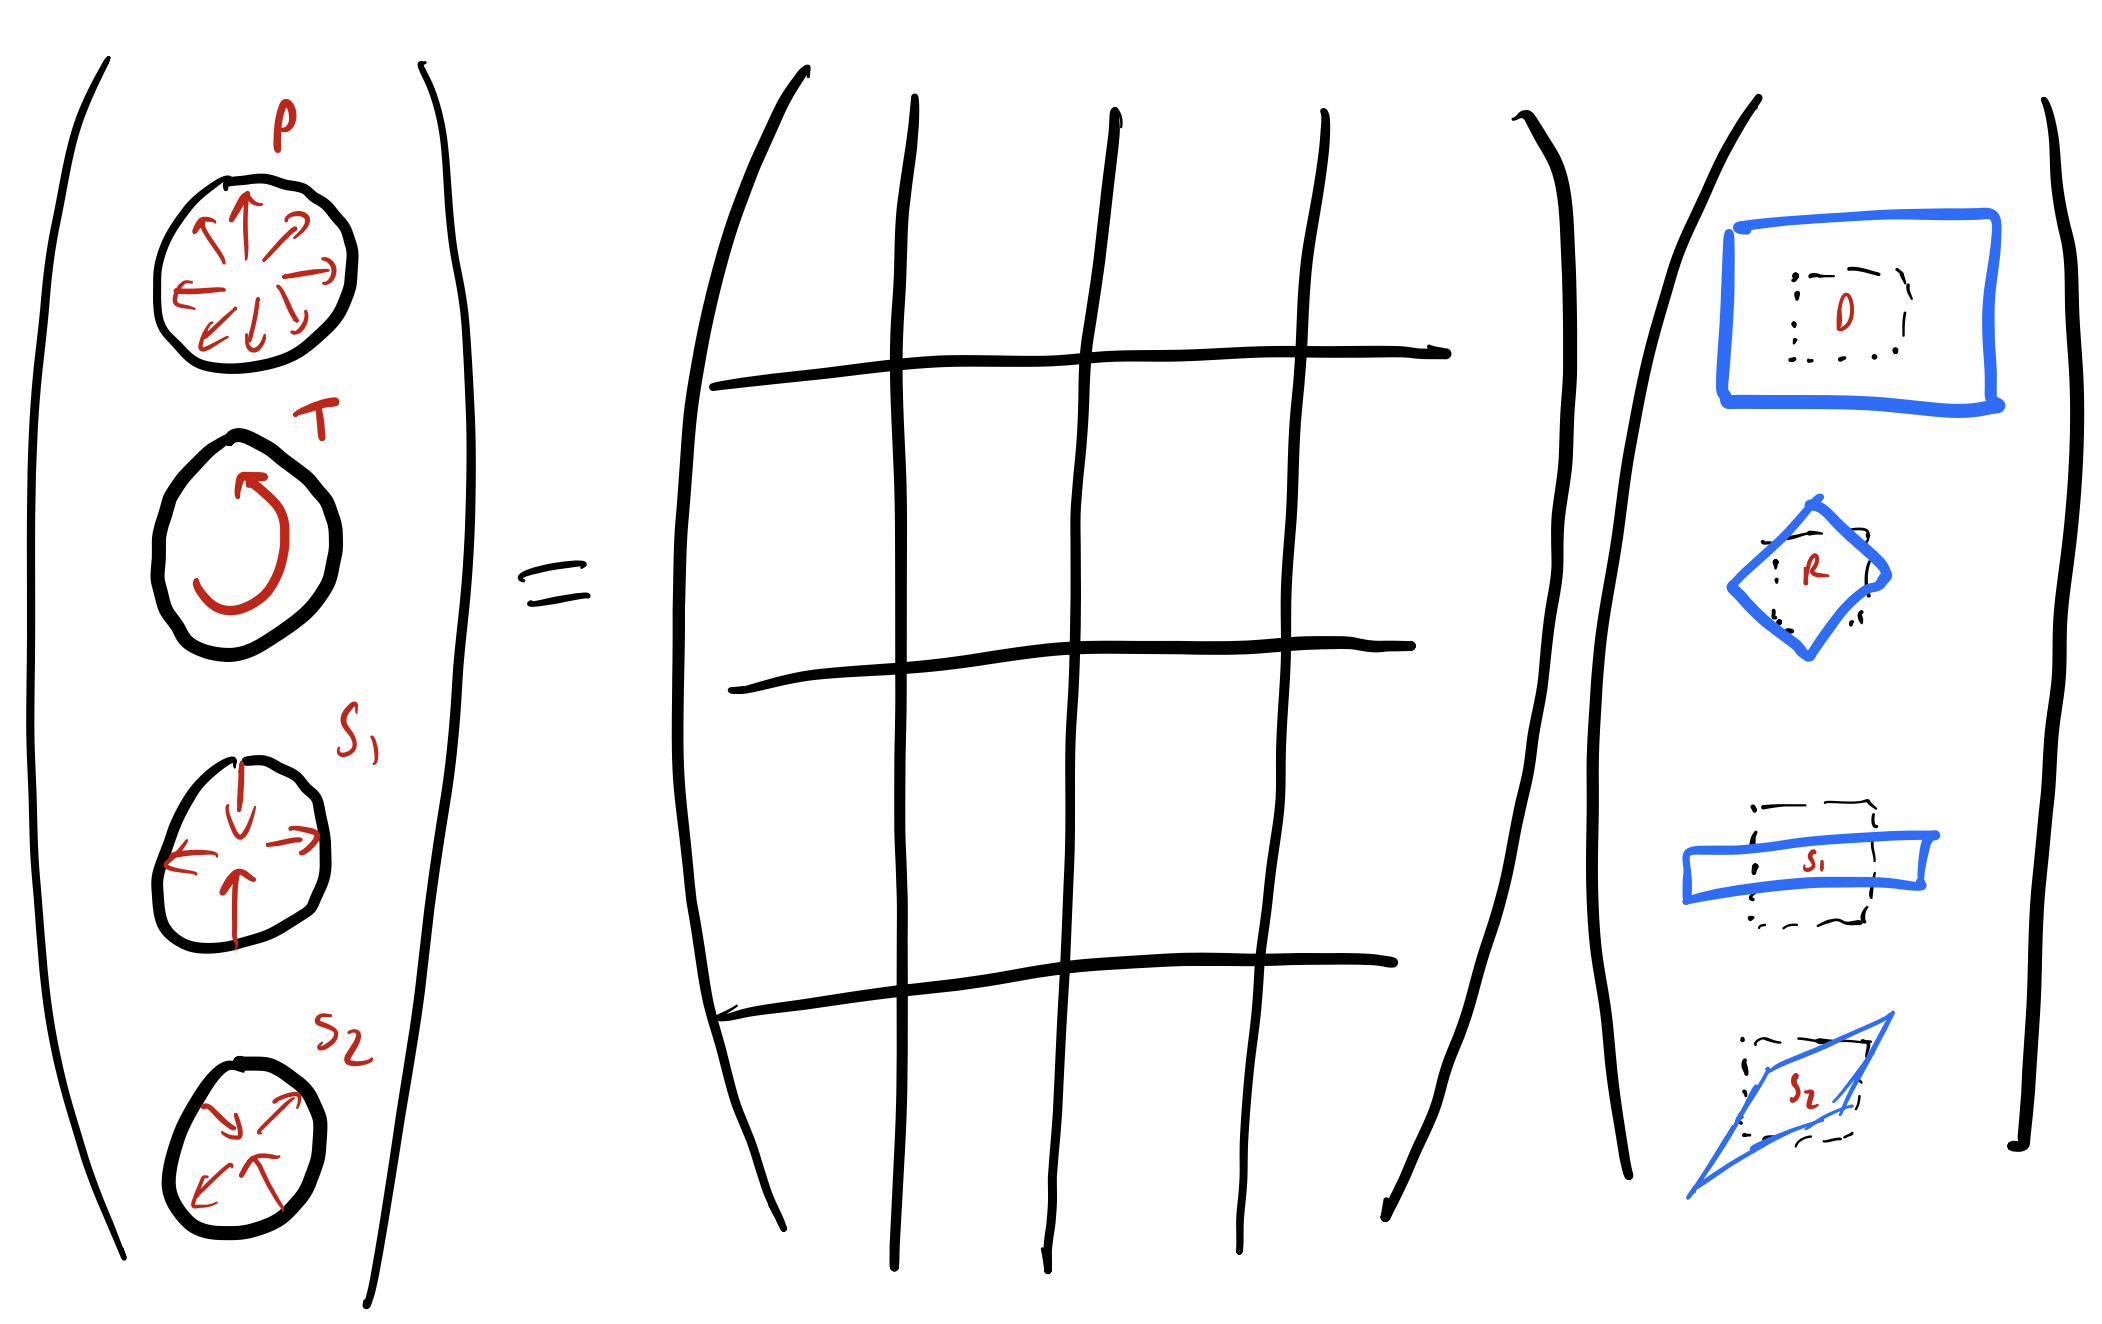
\includegraphics[scale=0.3]{Lectures/Images/lec2-stiffnessmatrix.png}
\end{center}
\begin{equation}
    \m{\text{P} \\ \text{T} \\ \text{SS1} \\ \text{SS2}} = \m{\cdot & \cdot & \cdot & \cdot \\ \cdot & \cdot & \cdot & \cdot \\ \cdot & \cdot & \cdot & \cdot \\ \cdot & \cdot & \cdot & \cdot}\m{\text{D} \\ \text{R} \\ \text{S1} \\ \text{S2}}
\end{equation}
This is really a statement about taking the stresses/strains and projecting on the group of matrices:
\begin{equation}
    \tau^0 = \m{1 & 0 \\ 0 & 1}, \quad \tau^1 = \m{0 & 1 \\ -1 & 0}, \quad \tau^2 = \m{1 & 0 \\ 0 & -1}, \quad \tau^3 = \m{0 & 1 \\ 1 & 0}
\end{equation}
where with this projection:
\begin{equation}
    \sigma^\alpha = \tau^\alpha_{ij}\sigma_{ij}
\end{equation}
\begin{equation}
    v^\beta = \tau_{ij}^\beta v_{ij}
\end{equation}
\begin{equation}
    \eta^{\alpha\beta} = \frac{1}{2}\tau^{\alpha}_{ij}K_{ijkl}\tau^\beta_{kl}
\end{equation}
Let us populate the entries of the matrix:
\begin{equation}
    \m{\text{P} \\ \text{T} \\ \text{SS1} \\ \text{SS2}} = \m{\xi & \cdot & 0 & 0 \\ \cdot & \cdot & 0 & 0 \\ 0 & 0 & \eta & \cdot \\ 0 & 0 & \cdot & \eta}\m{\text{D} \\ \text{R} \\ \text{S1} \\ \text{S2}}
\end{equation}
$\xi$ is the bulk viscosity, $\eta$ is the shear viscosity. The off diagonal blocks are assuming isotropy because we cannot connect the scalar and bivector parts. Further, the form of the rotation operator enforces the off diagonals to be zero (as the rotation operator forces that the odd diagonals are equal and opposite, and the symmetry of the matrix enforces that they are equal - hence they must be zero). So:
\begin{equation}
    \m{\text{P} \\ \text{T} \\ \text{SS1} \\ \text{SS2}} = \m{\xi & 0 & 0 & 0 \\ 0 & 0 & 0 & 0 \\ 0 & 0 & \eta & 0 \\ 0 & 0 & 0 & \eta}\m{\text{D} \\ \text{R} \\ \text{S1} \\ \text{S2}}
\end{equation}
If we now relax the $\eta_{\alpha\beta} = \eta_{\beta\alpha}$ condition so the matrix is not symmetric, in the lower diagonal block and upper diagonal block we can introduce new terms, as well as a rotation term:
\begin{equation}
    \m{\text{P} \\ \text{T} \\ \text{SS1} \\ \text{SS2}} = \m{\xi & \eta^B & 0 & 0 \\ \eta^A & \eta^R & 0 & 0 \\ 0 & 0 & \eta & \eta^0 \\ 0 & 0 & -\eta^0 & \eta}\m{\text{D} \\ \text{R} \\ \text{S1} \\ \text{S2}}
\end{equation}
Rotational invariance would set $\eta^B = \eta^R = 0$, but even with this assumption $\eta^A$ would persist. What remains is completely analogous to the $A, K^0$ coefficients that arose in our discussion of odd elasticity.

The interpretation of $\eta^A$ is depending on the rate at which you can compress, there is a torque in response. If you know that your fluid has zero torque density, then it vanishes. The odd elasticity equivalent was the robots with a bond-bending angle, which had $K^0$ but no $A$. $\eta_As$ can only exist if $\sigma_{ij} \neq \sigma_{ji}$.

\subsection{Equations - Tensorial Form}
Instead of writing things in this intuitive notation, we can also write things down in tensorial notation (like we did for $K_{ijl}$), which is generally more useful for calculations. Let us write:
\begin{equation}
    \eta_{ijkl} = \xi \delta_{ij}\delta_{kl} - \eta^A \e_{ij}\delta_{mn} - \eta^B \delta_{ij}\e_{kl} + \eta^R \e_{ij}\e_{kl} + \eta(\delta_{il}\delta_{jk} + \delta_{ik}\delta_{jl} - \delta_{ij}\delta_{kl}) + \eta^0\frac{1}{2}(\e_{ik}\delta_{jl} + \e_{il}\delta_{jk} + \e_{jk}\delta_{il} + \e_{jl}\delta_{ik})
\end{equation}
The latter two look complicated, but you can check that $\eta_{ijkl} = \eta_{klij}$ for the even term and $\eta_{ijkl} = -\eta_{klij}$ for the odd term.

If we were to add a pressure or pre-torque through $\sigma^h$, the above is modified to be:
\begin{equation}
        \m{\text{P} \\ \text{T} \\ \text{SS1} \\ \text{SS2}} = \m{\xi & \eta^B & 0 & 0 \\ \eta^A & \eta^R & 0 & 0 \\ 0 & 0 & \eta & \eta^0 \\ 0 & 0 & -\eta^0 & \eta}\m{\text{D} \\ \text{R} \\ \text{S1} \\ \text{S2}} + \m{-p \\ -\tau \\ 0 \\ 0}
\end{equation}
Now, taking this definition of $\sigma_{ij}$, we can put it into the Navier-Stokes equation:
\begin{equation}
    \rho D_t \v{v} = \underbrace{\nabla \sigma^h}_{=0} + \xi\nabla(\nabla \cdot \v{v}) + \underbrace{\eta\nabla^2\v{v}}_{\eta\p_k \p_k v_i} + \underbrace{\eta^0\e \cdot \nabla^2 \v{v}}_{\eta^0\e_{ij}\p_k\p_k v_j} - \eta^A \e \cdot\nabla(\nabla \cdot \v{v}) + \eta^B \nabla(\nabla \times \v{v}) - \eta^R \e \cdot \nabla(\nabla \times \v{v})
\end{equation}
Next time, we remove some terms, and study a fluid with just $\eta, \eta^0$ terms in 2-D. We then progress to more complicated settings of 3-D and fluids with turbulence.